\documentclass[tikz,border=6pt]{standalone}
\usepackage{amsmath,amssymb}
\usetikzlibrary{arrows.meta,decorations.pathreplacing}

\begin{document}
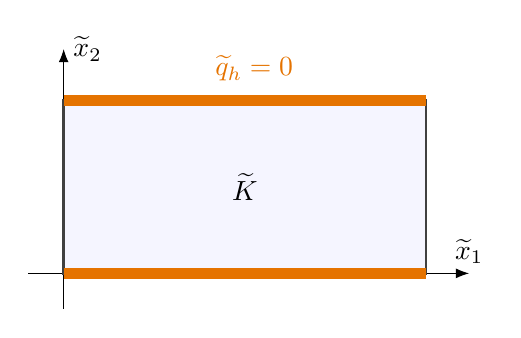
\begin{tikzpicture}[x=1cm,y=1cm,>=Latex]
  \coordinate (A) at (0,0);
  \coordinate (B) at (0,2.2);
  \coordinate (C) at (4.6,2.2);
  \coordinate (D) at (4.6,0);

  \draw[->] (-0.45,0) -- (5.15,0) node[above] {$\widetilde x_1$};
  \draw[->] (0,-0.45) -- (0,2.85) node[right] {$\widetilde x_2$};

  \fill[blue!4] (A) rectangle (C);
  \draw[line width=0.9pt,black!75] (A) rectangle (C);
  \draw[line width=4pt,orange!90!black] (A) -- (D);
  \draw[line width=4pt,orange!90!black] (B) -- (C);

  \node at (2.3,1.1) {$\widetilde K$};
  \node[orange!90!black] at (2.42,2.6) {$\widetilde q_h=0$};
\end{tikzpicture}
\end{document}
